%%% Walker and Trace Plots

%%% Nobin
\begin{figure}
	\centering
	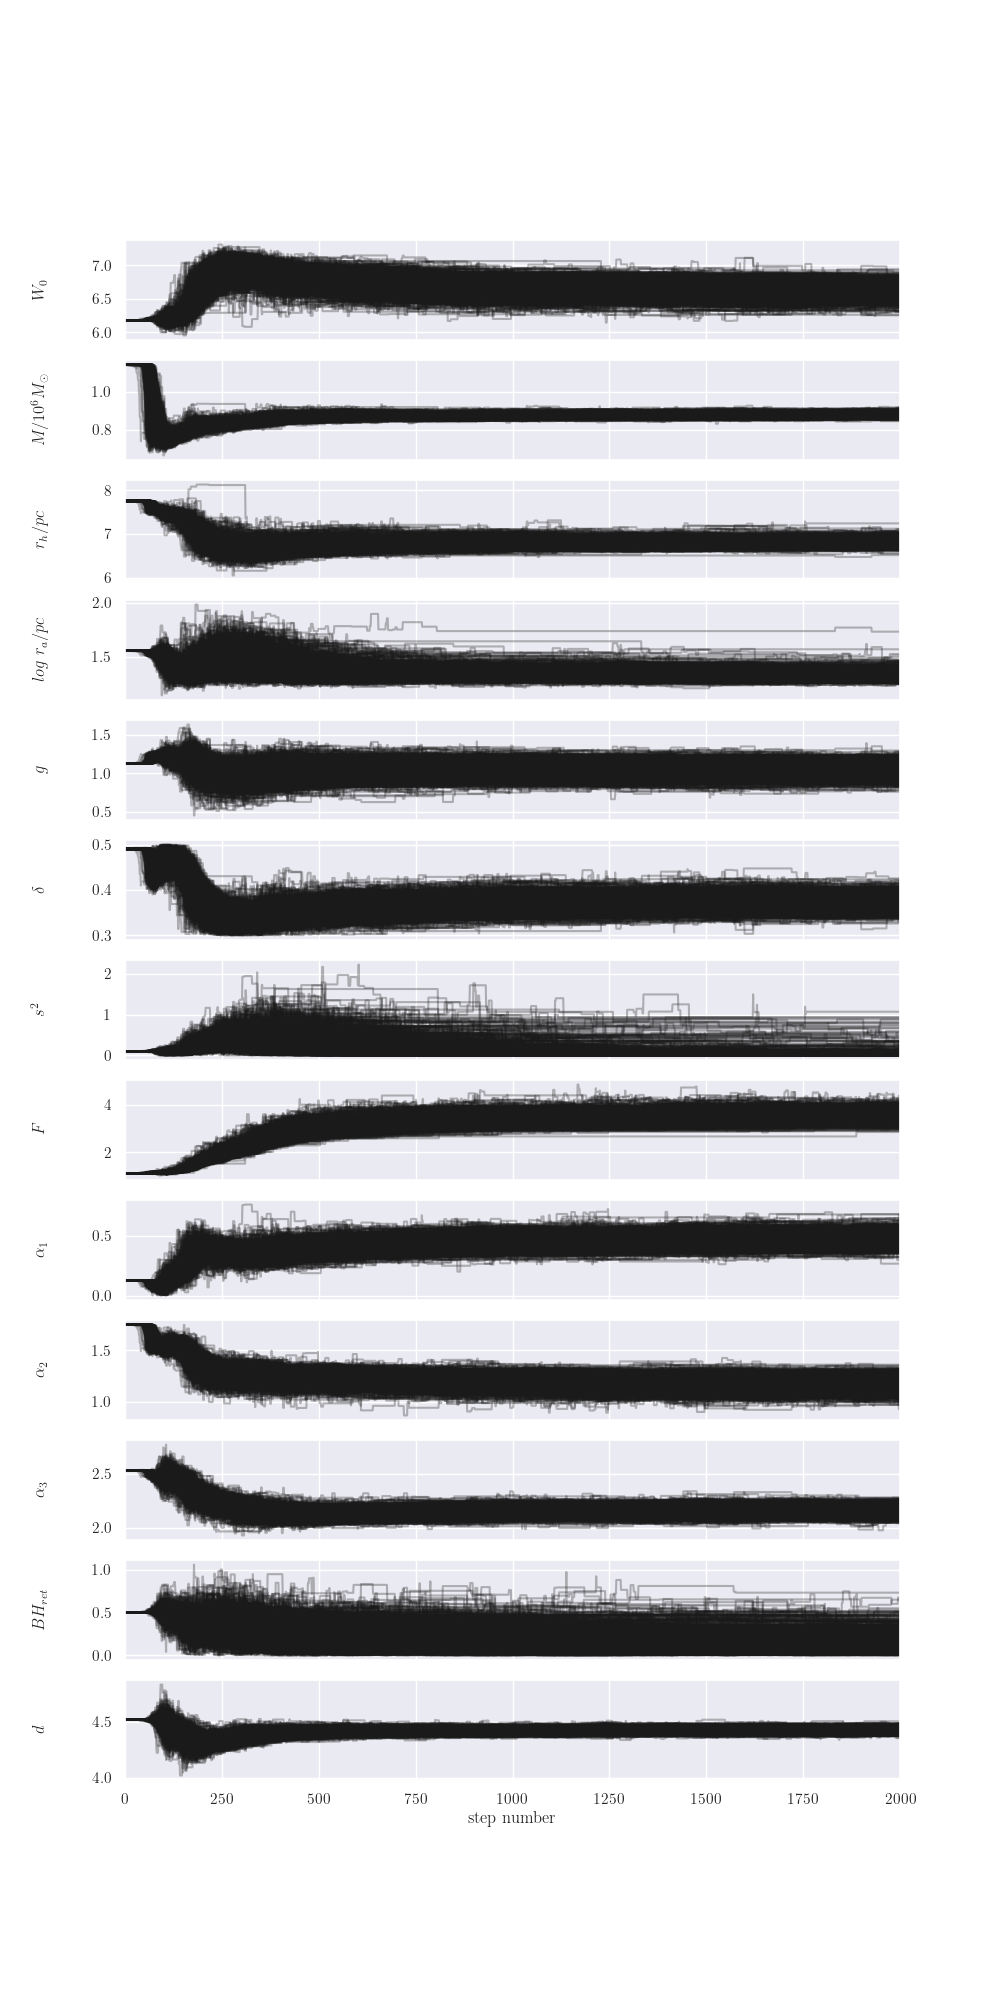
\includegraphics[width=0.7\textwidth]{figures/prev_nobin/walkers.png}
	\caption{Trace plot showing the evolution of the MCMC chain for model with a $0\%$ binary
		fraction.}
	\label{fig:nobin_walkers}
\end{figure}

\begin{figure}
	\centering
	\includegraphics[width=\textwidth]{figures/prev_nobin/corner.png}
	\caption{Corner plot showing the marginalized posterior probability distributions of models
		parameters with a $0\%$ binary fraction.}
	\label{fig:nobin_corner}
\end{figure}


%%% Lowbin
\begin{figure}
	\centering
	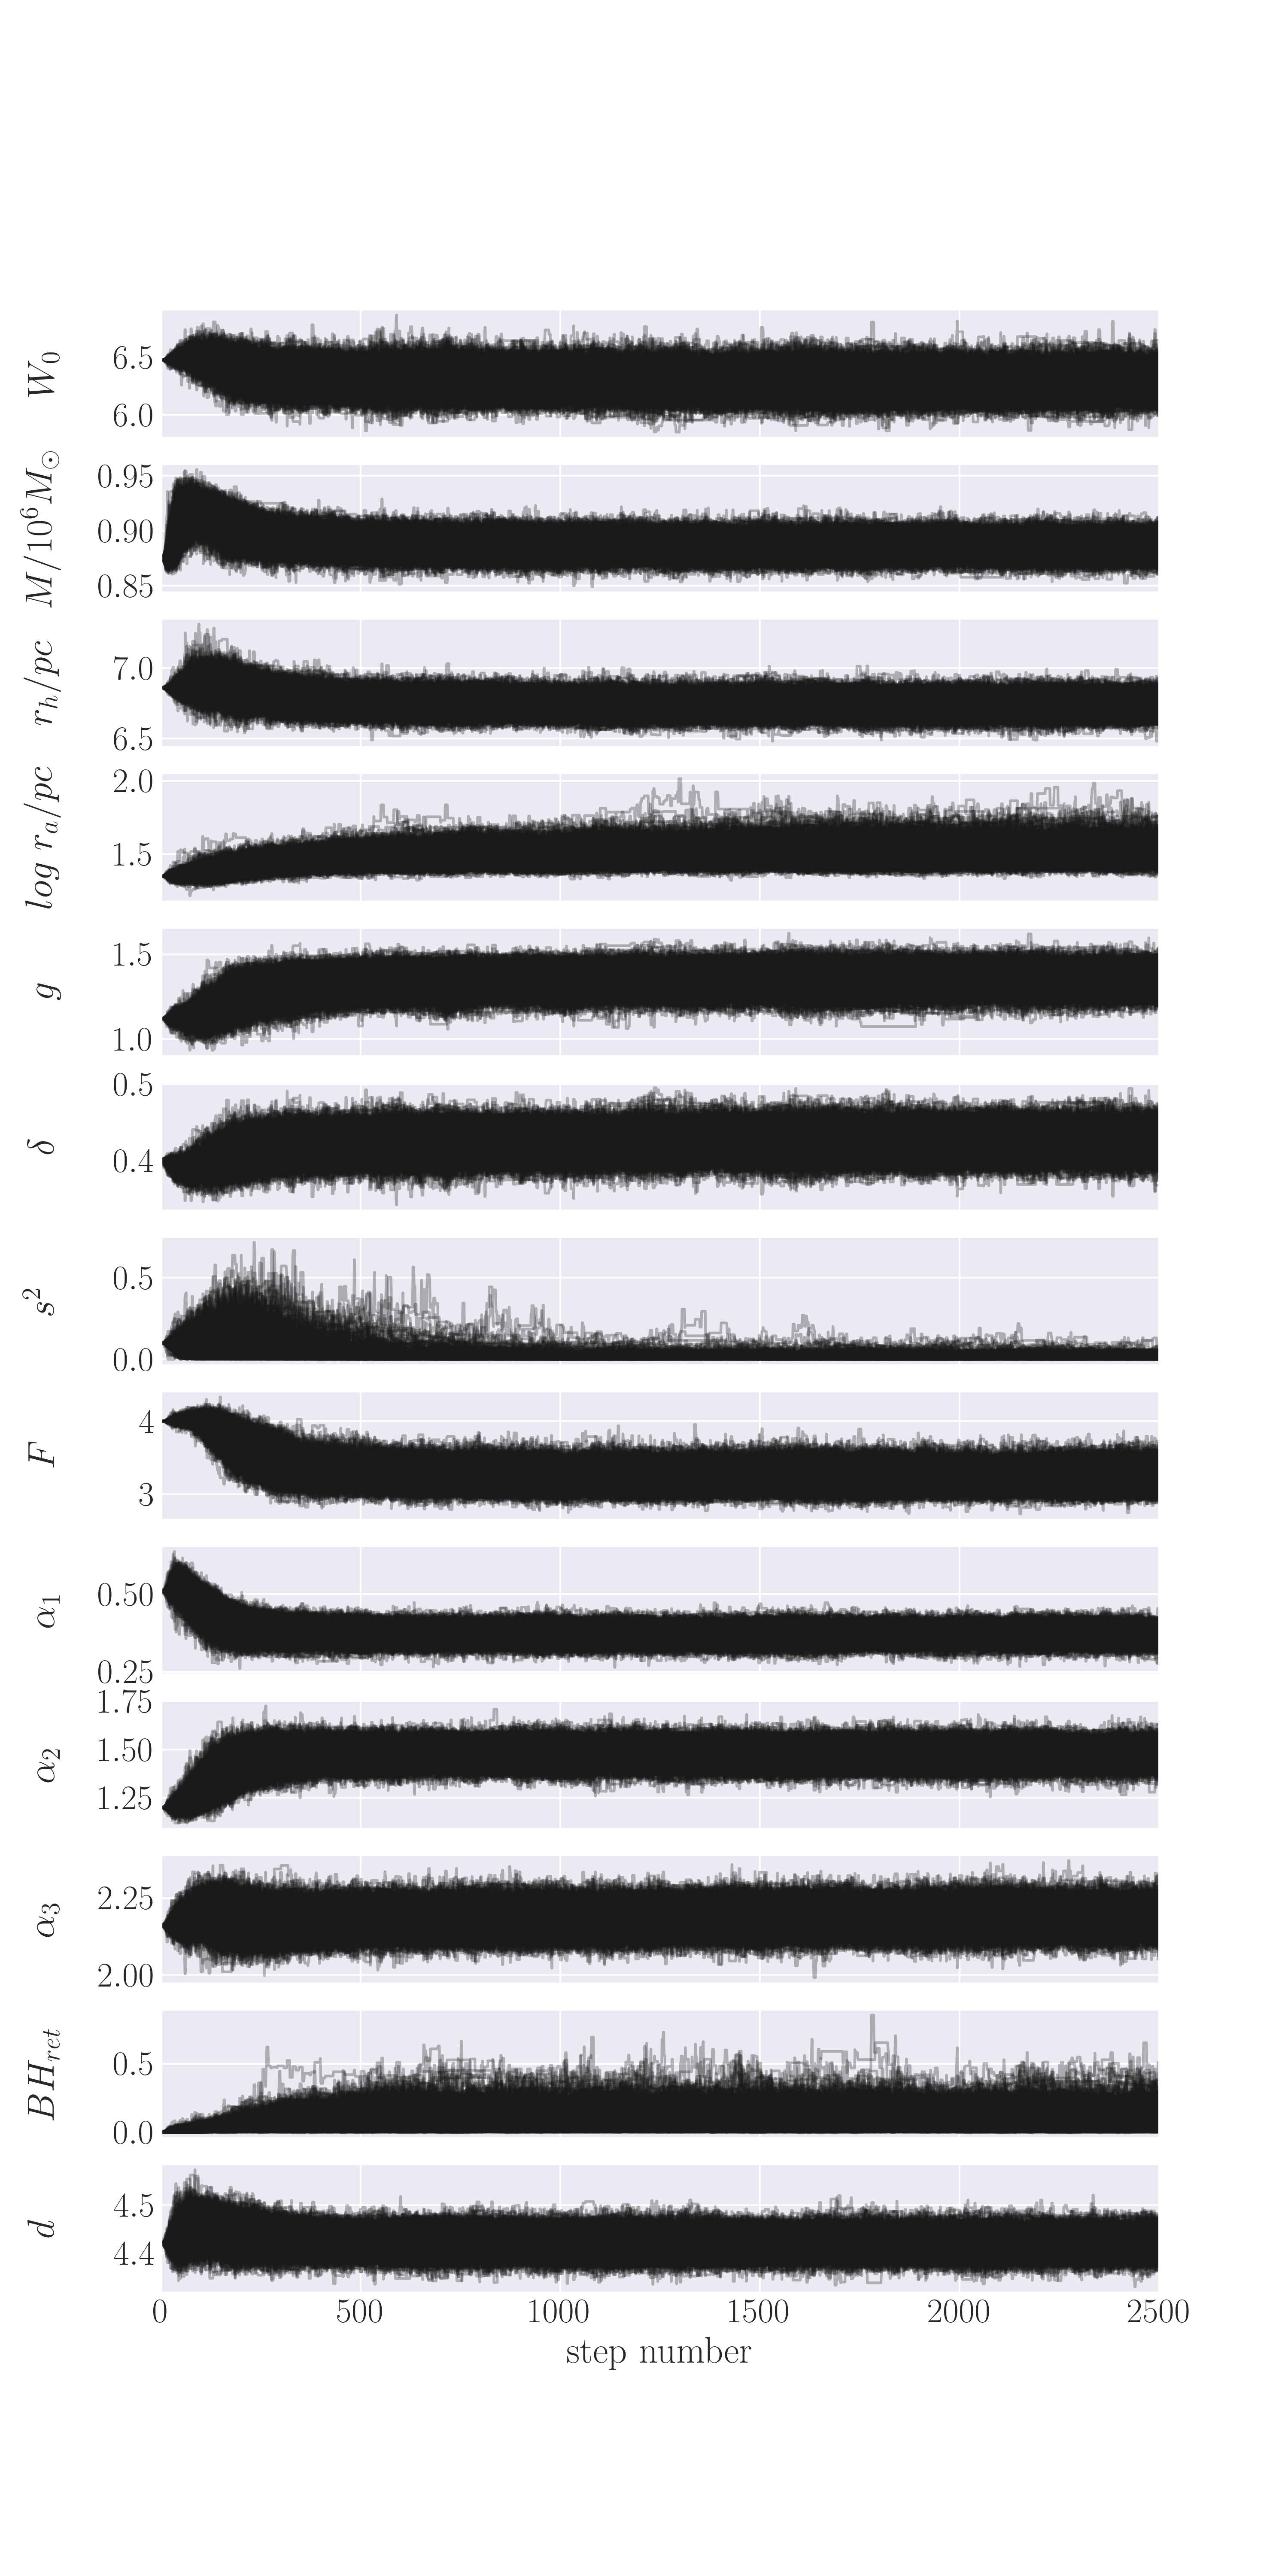
\includegraphics[width=0.7\textwidth]{figures/low_bin_model/walkers.png}
	\caption{Trace plot showing the evolution of the MCMC chain for model with a $2\%$ binary
		fraction.}
	\label{fig:lowbin_walkers}
\end{figure}

\begin{figure}
	\centering
	\includegraphics[width=\textwidth]{figures/low_bin_model/corner.png}
	\caption{Corner plot showing the marginalized posterior probability distributions of models
		parameters with a $2\%$ binary fraction.}
	\label{fig:lowbin_corner}
\end{figure}



%%% Highbin
\begin{figure}
	\centering
	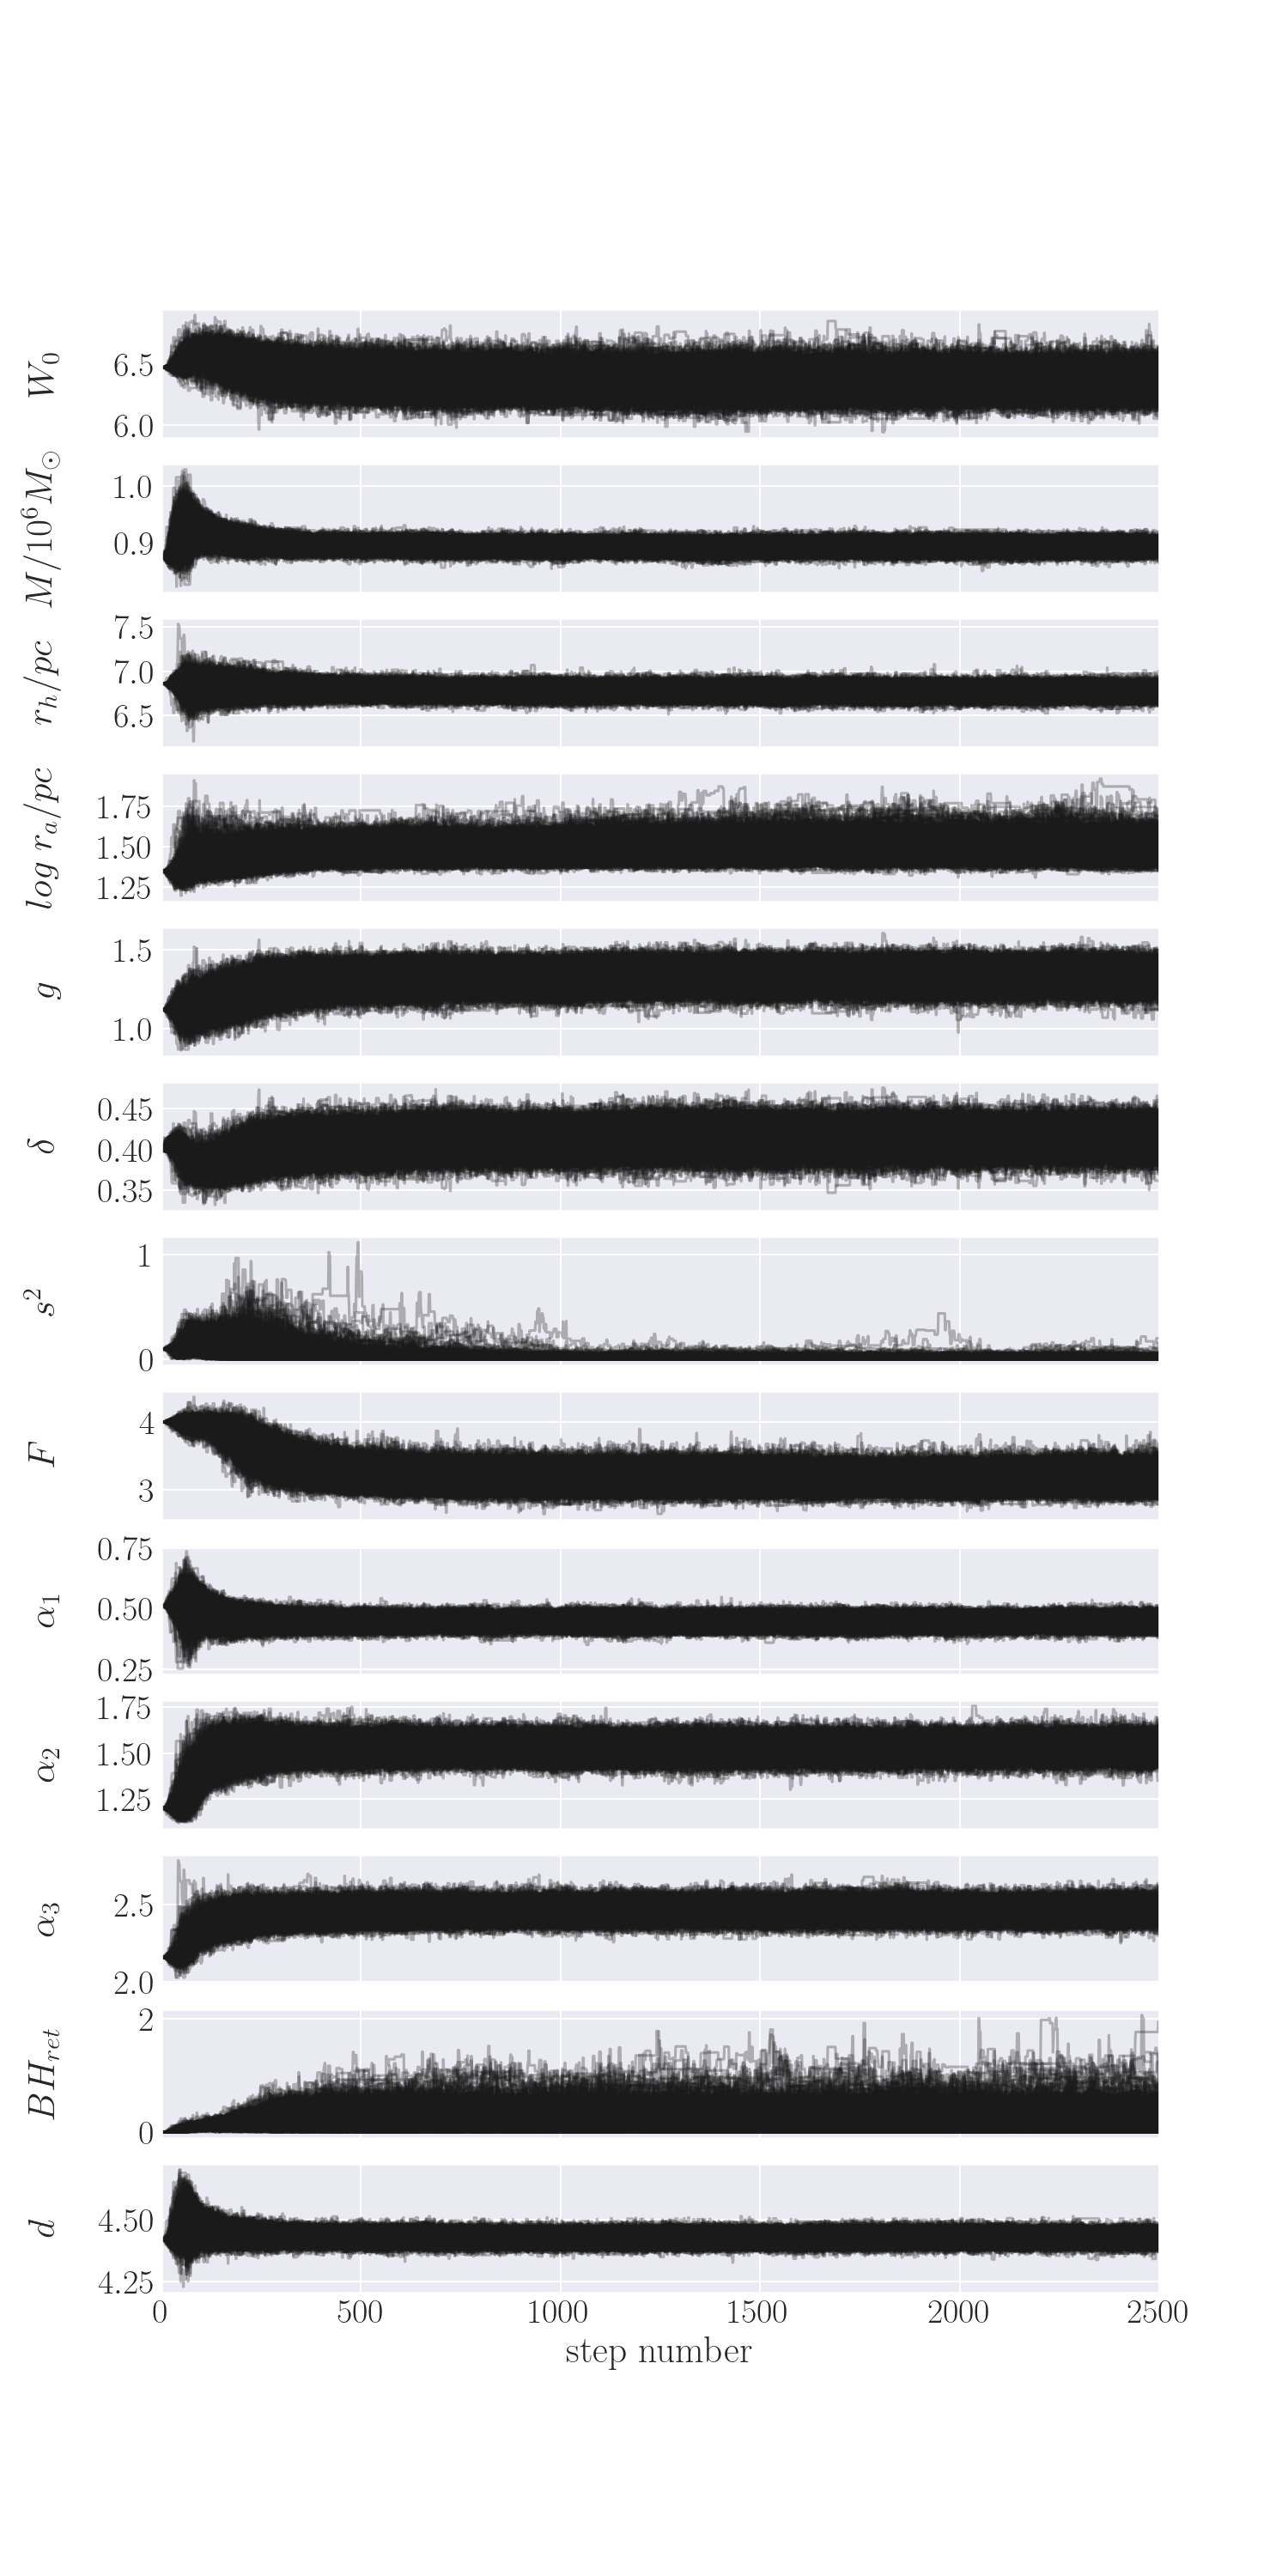
\includegraphics[width=0.7\textwidth]{figures/high_bin_model/walkers.png}
	\caption{Trace plot showing the evolution of the MCMC chain for model with a $10\%$ binary
		fraction.}
	\label{fig:highbin_walkers}
\end{figure}

\begin{figure}
	\centering
	\includegraphics[width=\textwidth]{figures/high_bin_model/corner.png}
	\caption{Corner plot showing the marginalized posterior probability distributions of models
		parameters with a $10\%$ binary fraction.}
	\label{fig:highbin_corner}
\end{figure}




%%% More Obs plots


%%% Nobin
\begin{figure}
	\begin{center}
		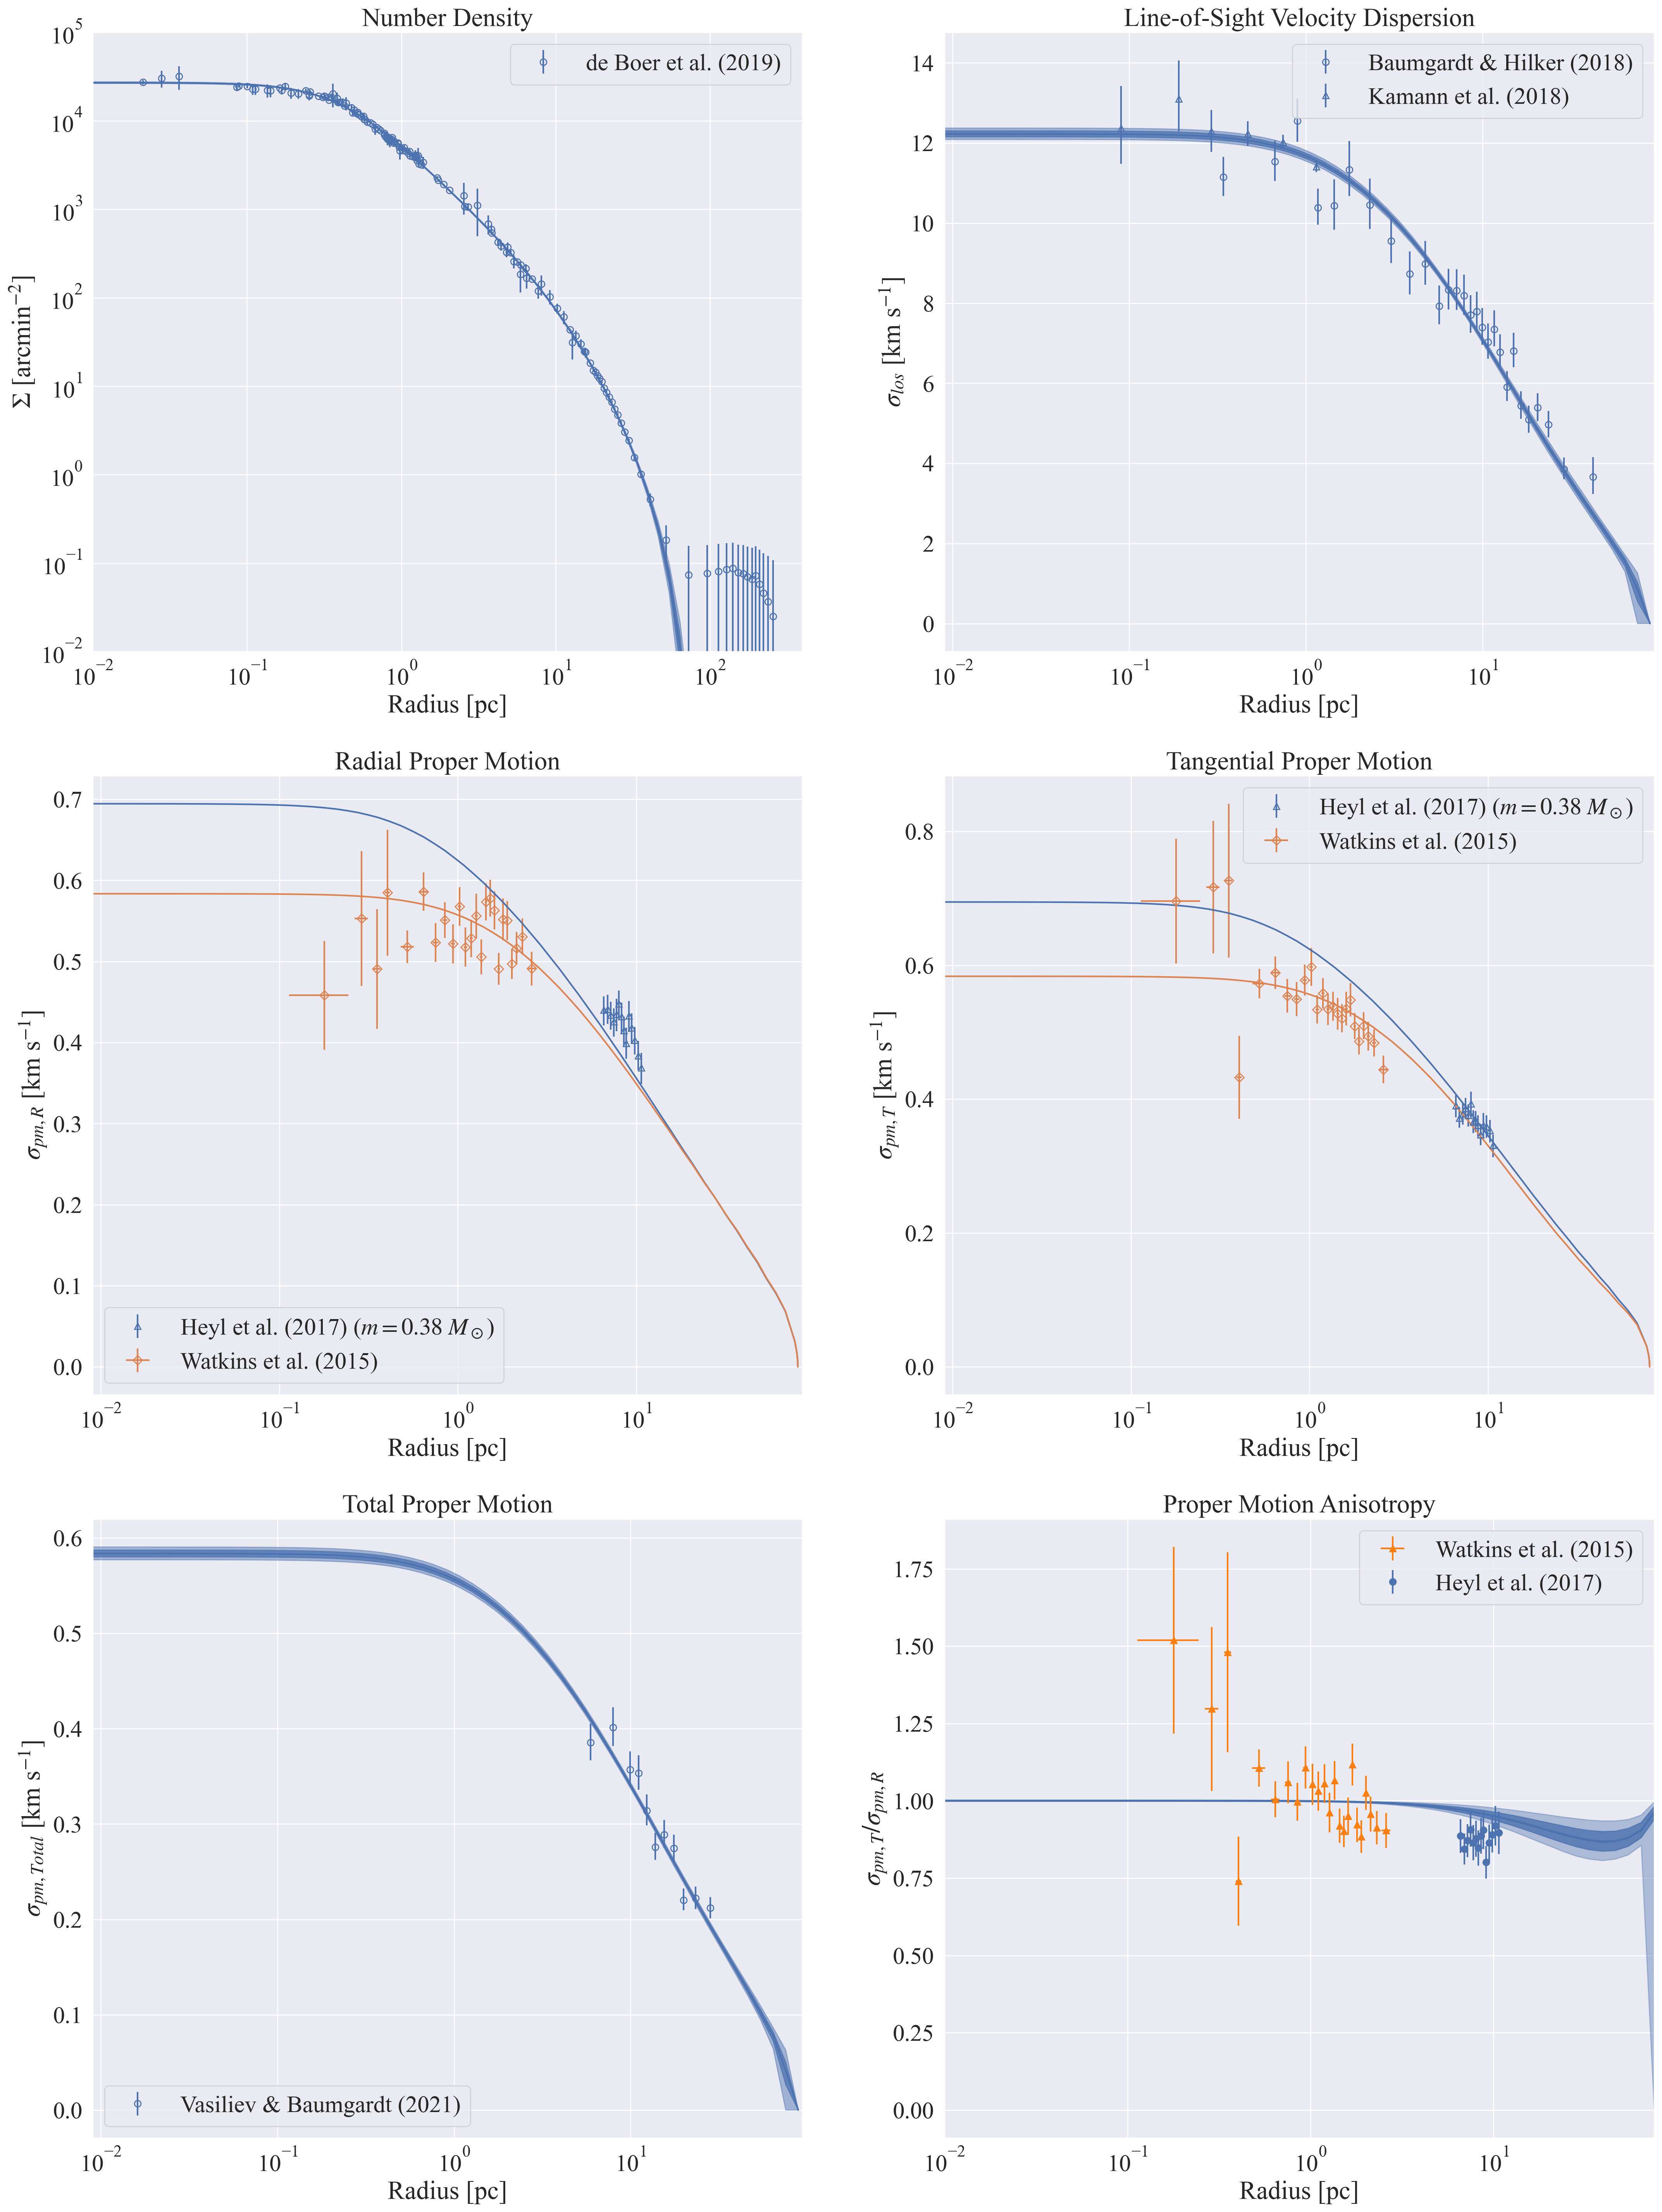
\includegraphics[width=0.9\textwidth]{figures/prev_nobin/obs_panel.png}
	\end{center}
	\caption{Model fits to the observables for models with no binary stars.}
	\label{fig:nobin_obs_panel}
\end{figure}

\begin{figure}
	\begin{center}
		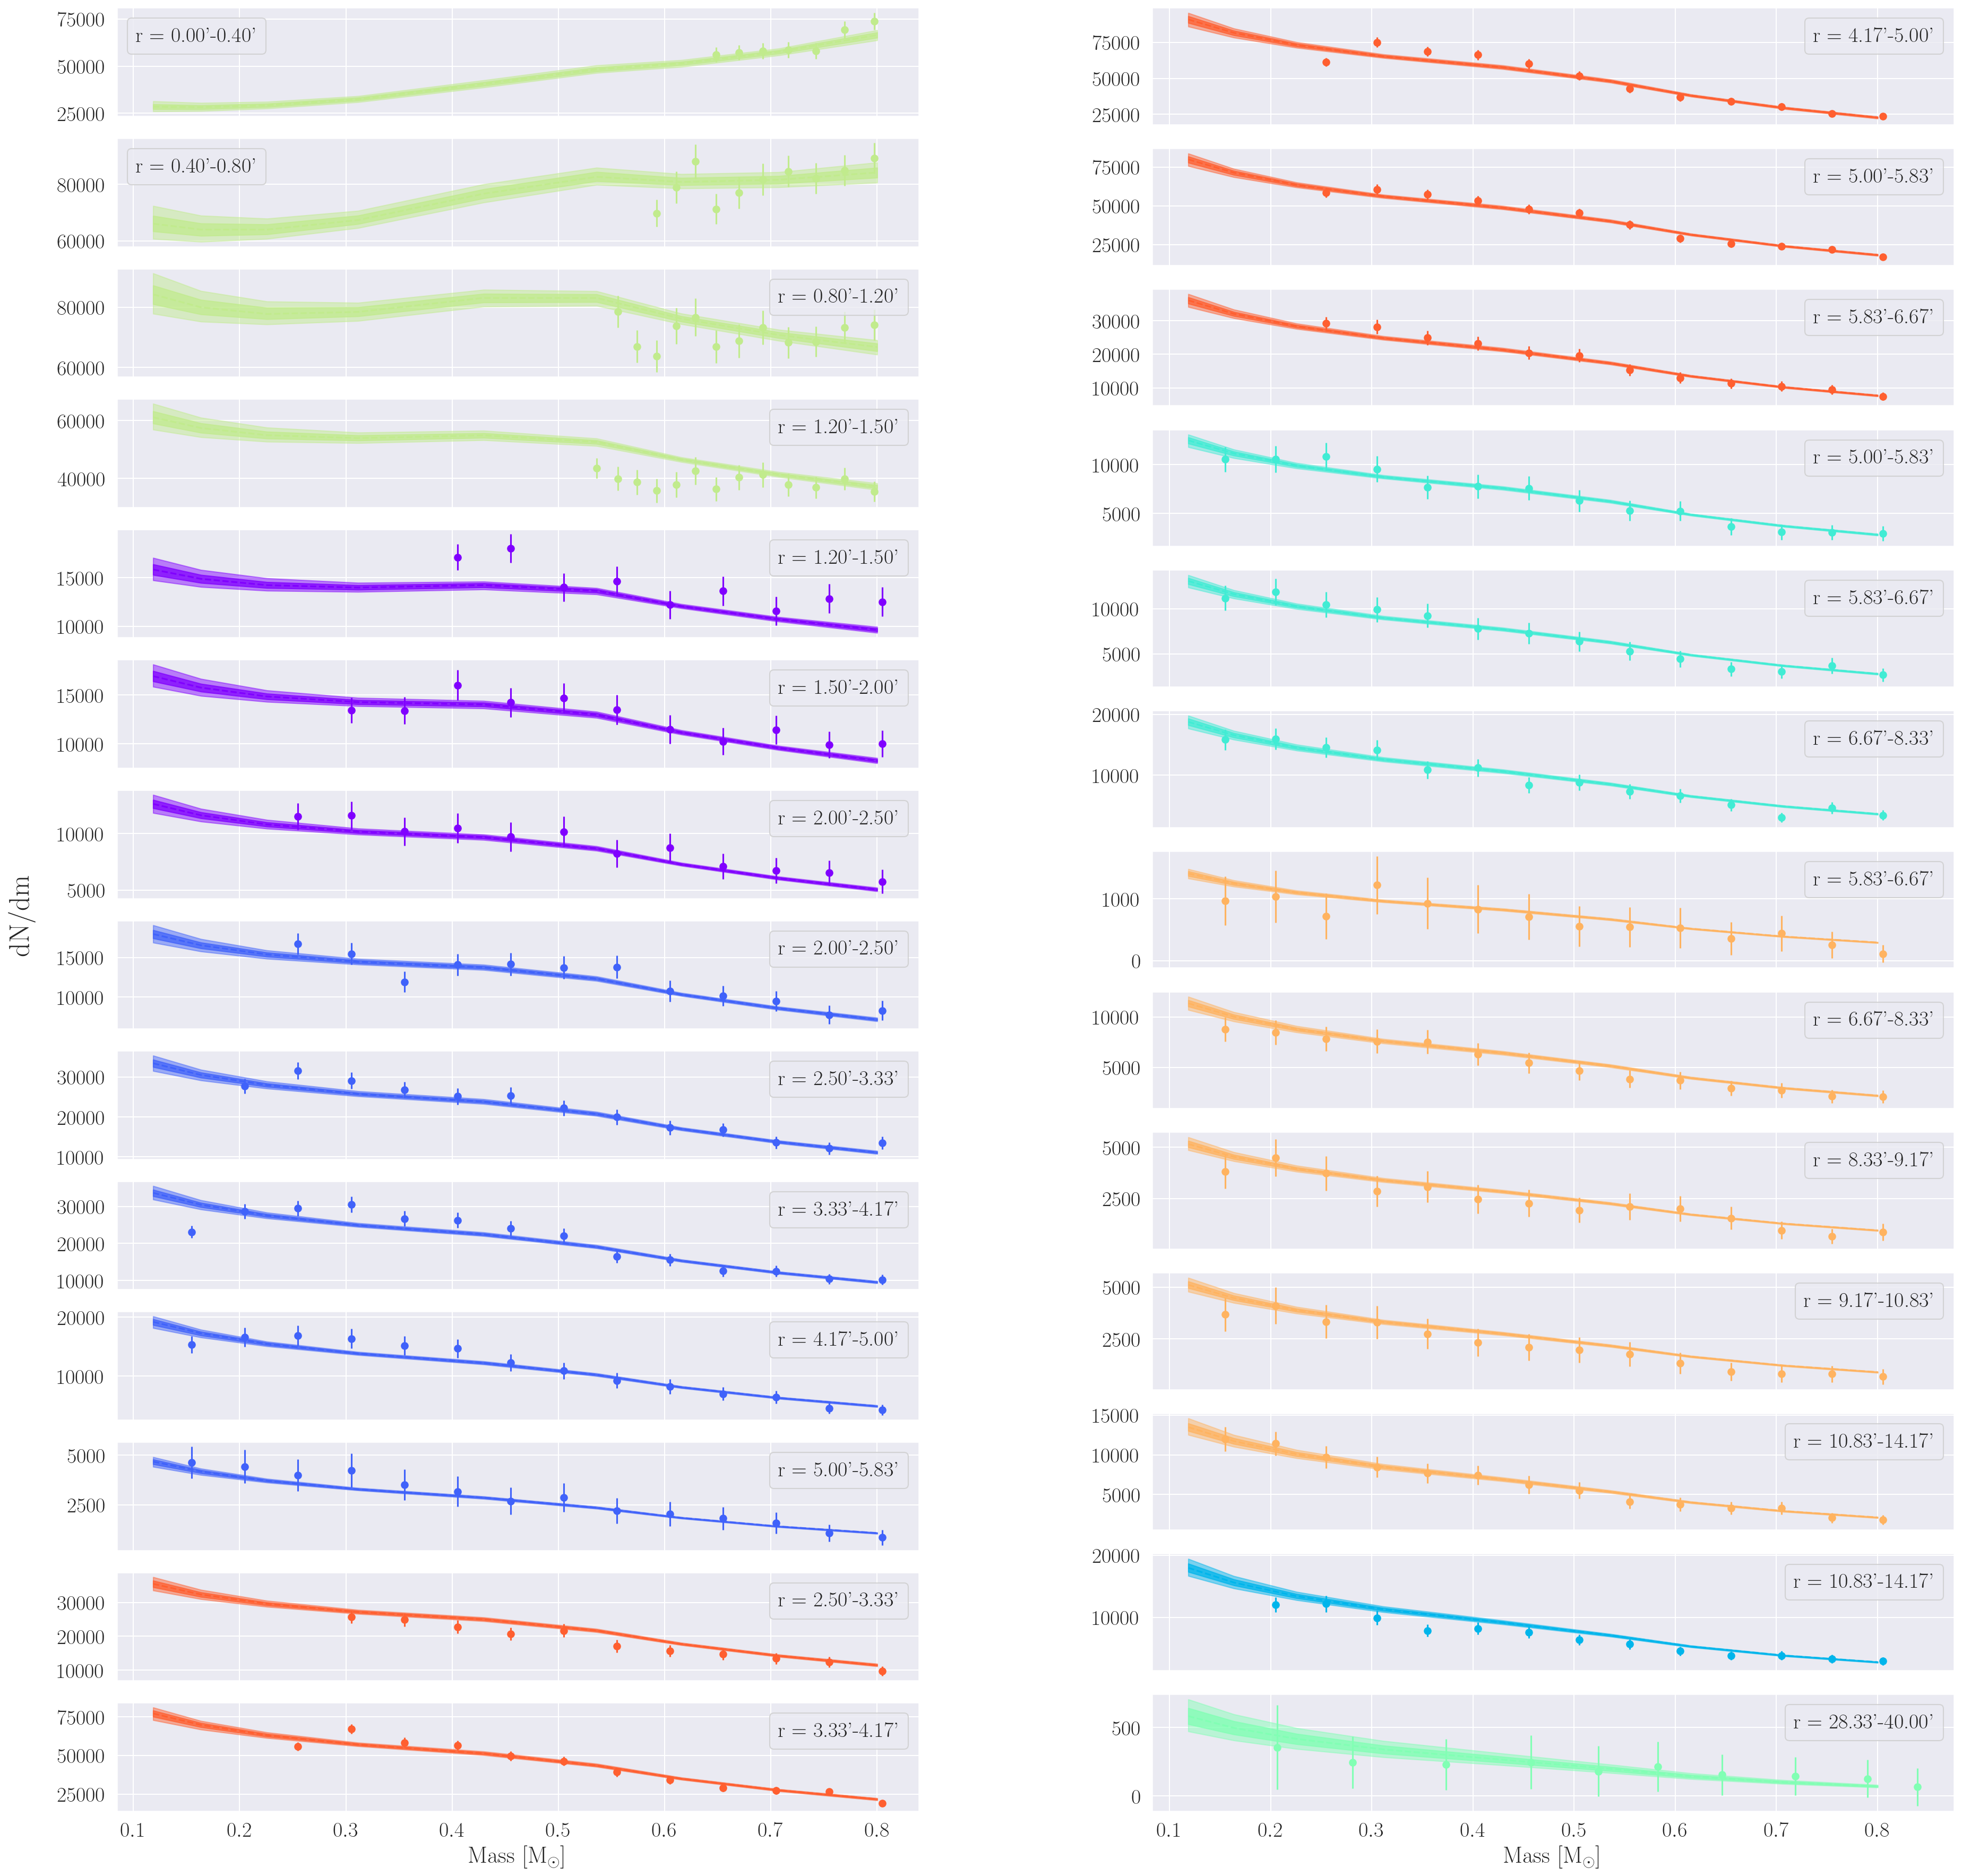
\includegraphics[width=0.9\textwidth]{figures/prev_nobin/mass_fun.png}
	\end{center}
	\caption{Model fits to stellar mass function data for models with no binary stars.}
	\label{fig:nobin_mass_fun}
\end{figure}


%%% Highbin
\begin{figure}
	\centering
	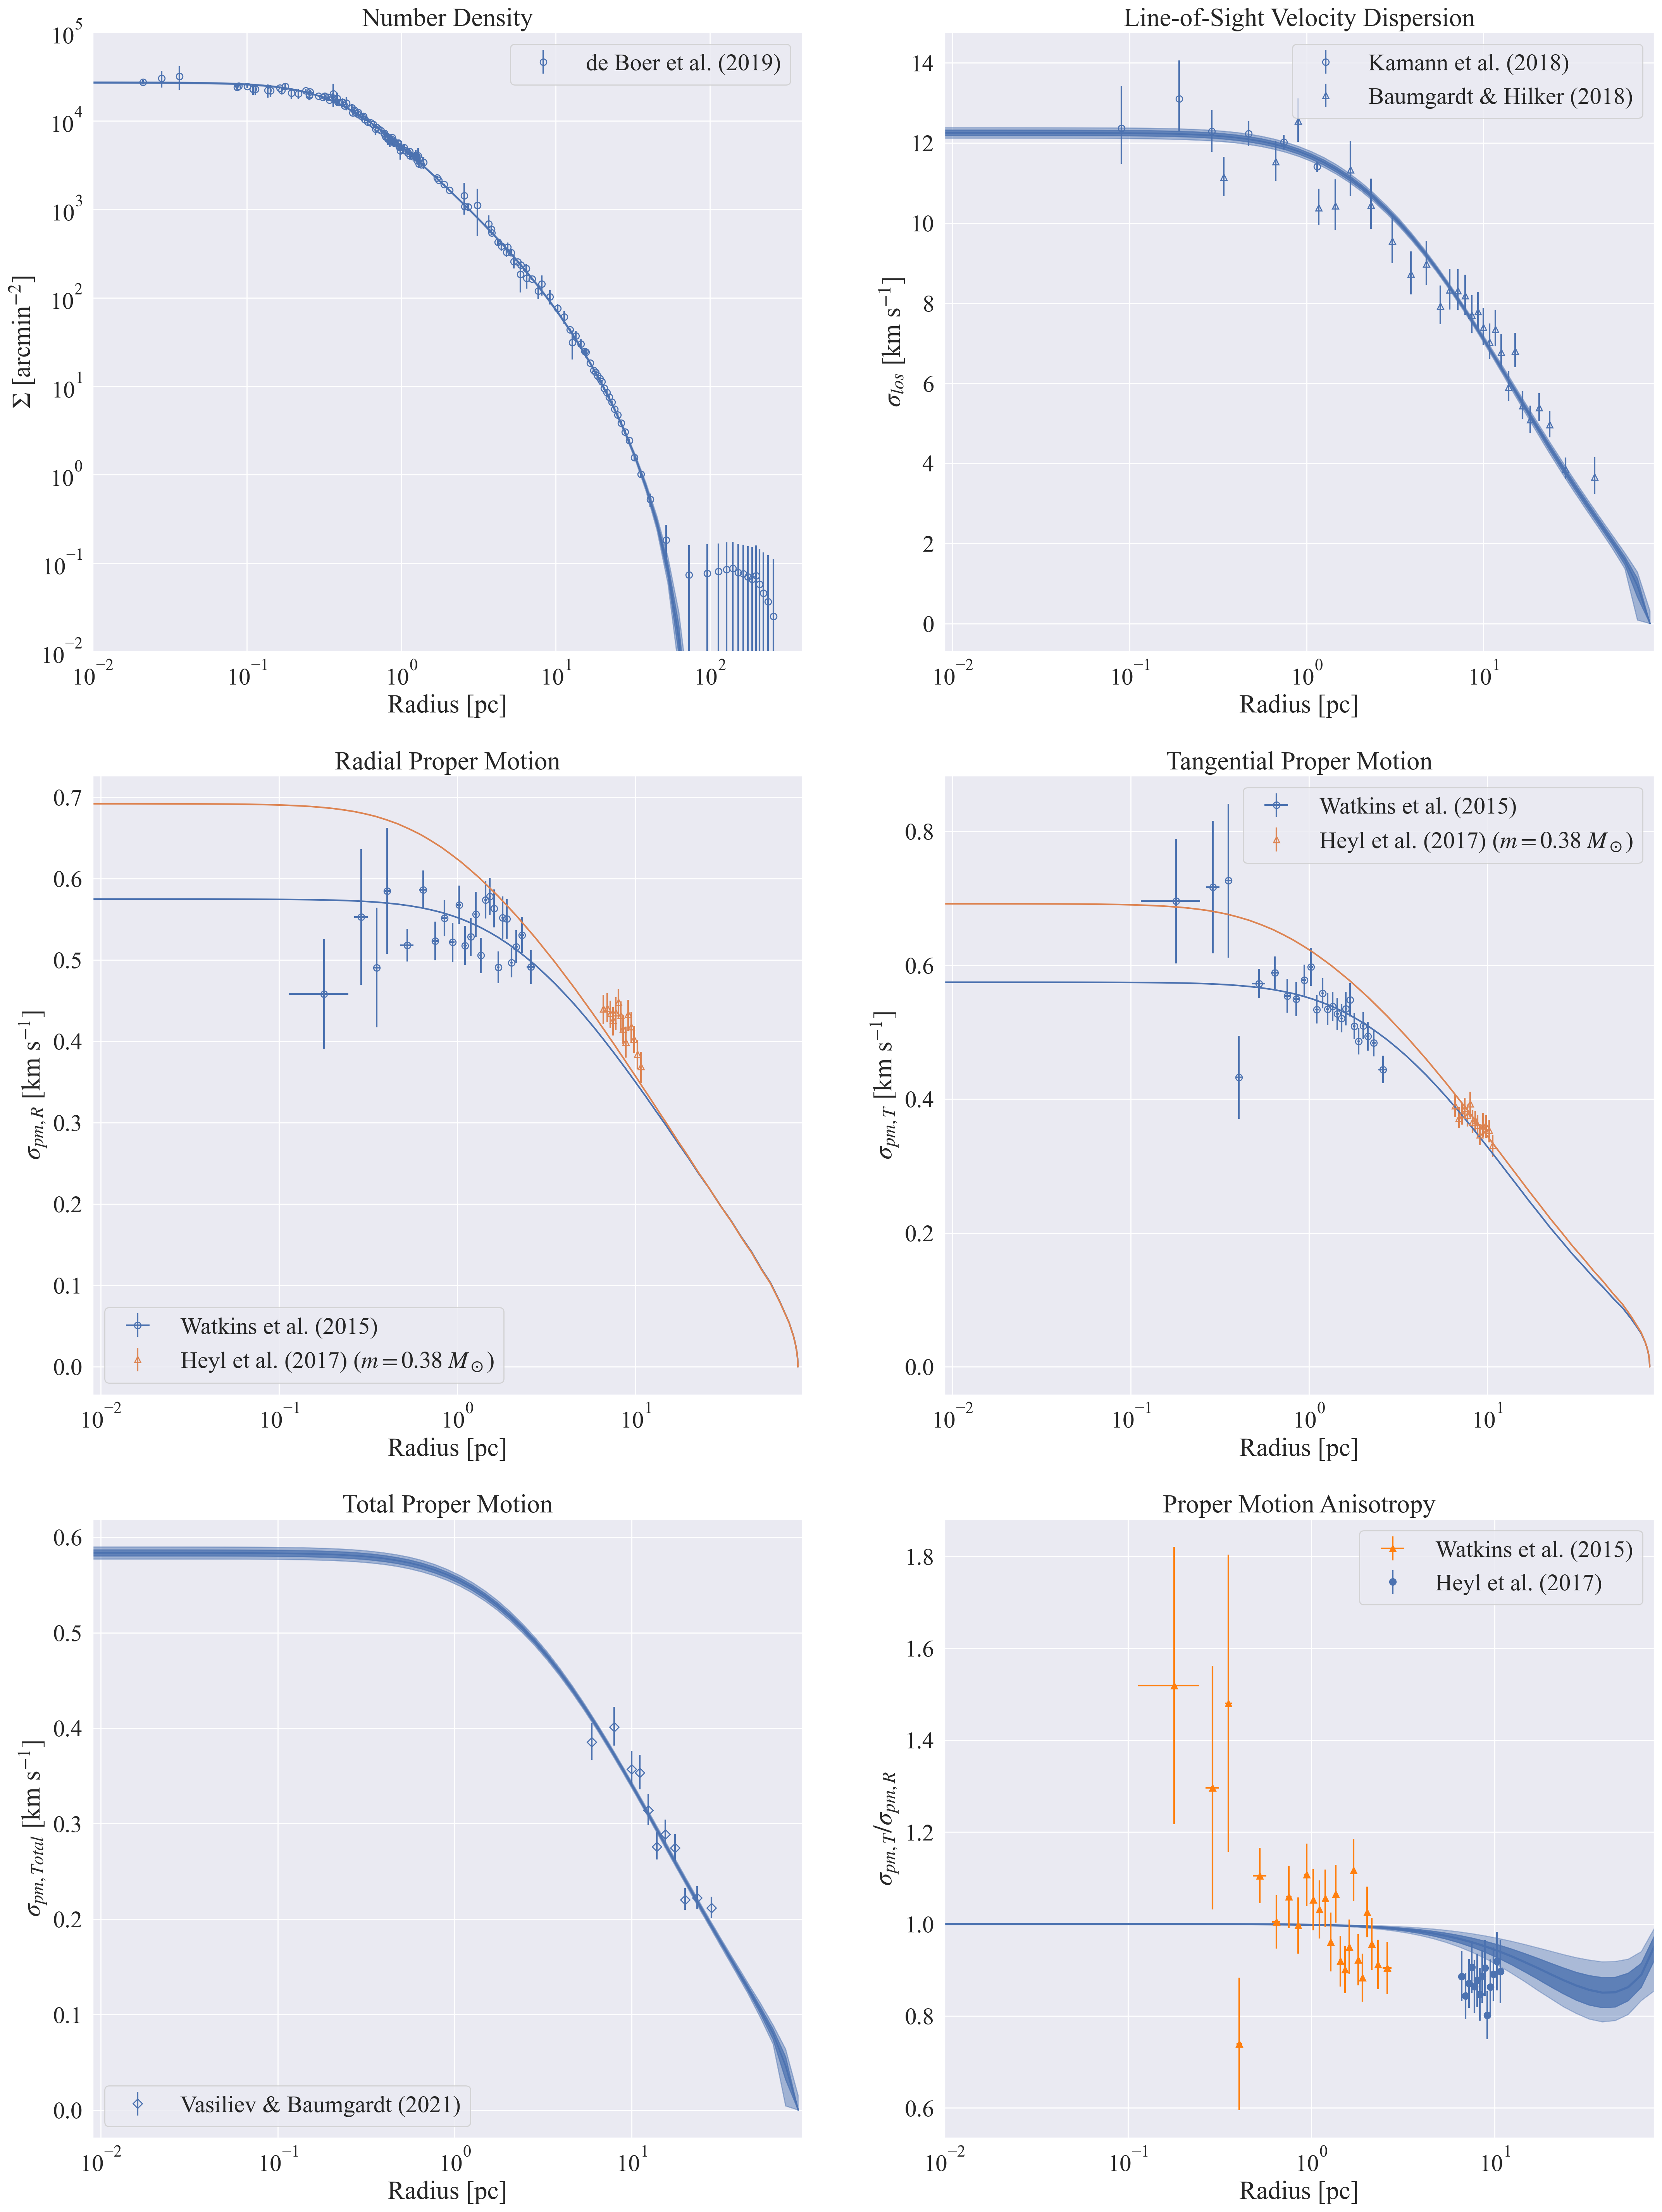
\includegraphics[width=0.8\textwidth]{figures/high_bin_model/obs_panel.png}
	\caption{Model fits to the observables for models with a $10\%$ binary fraction.}
	\label{fig:highbin_obs_panel}
\end{figure}


\begin{figure}
	\centering
	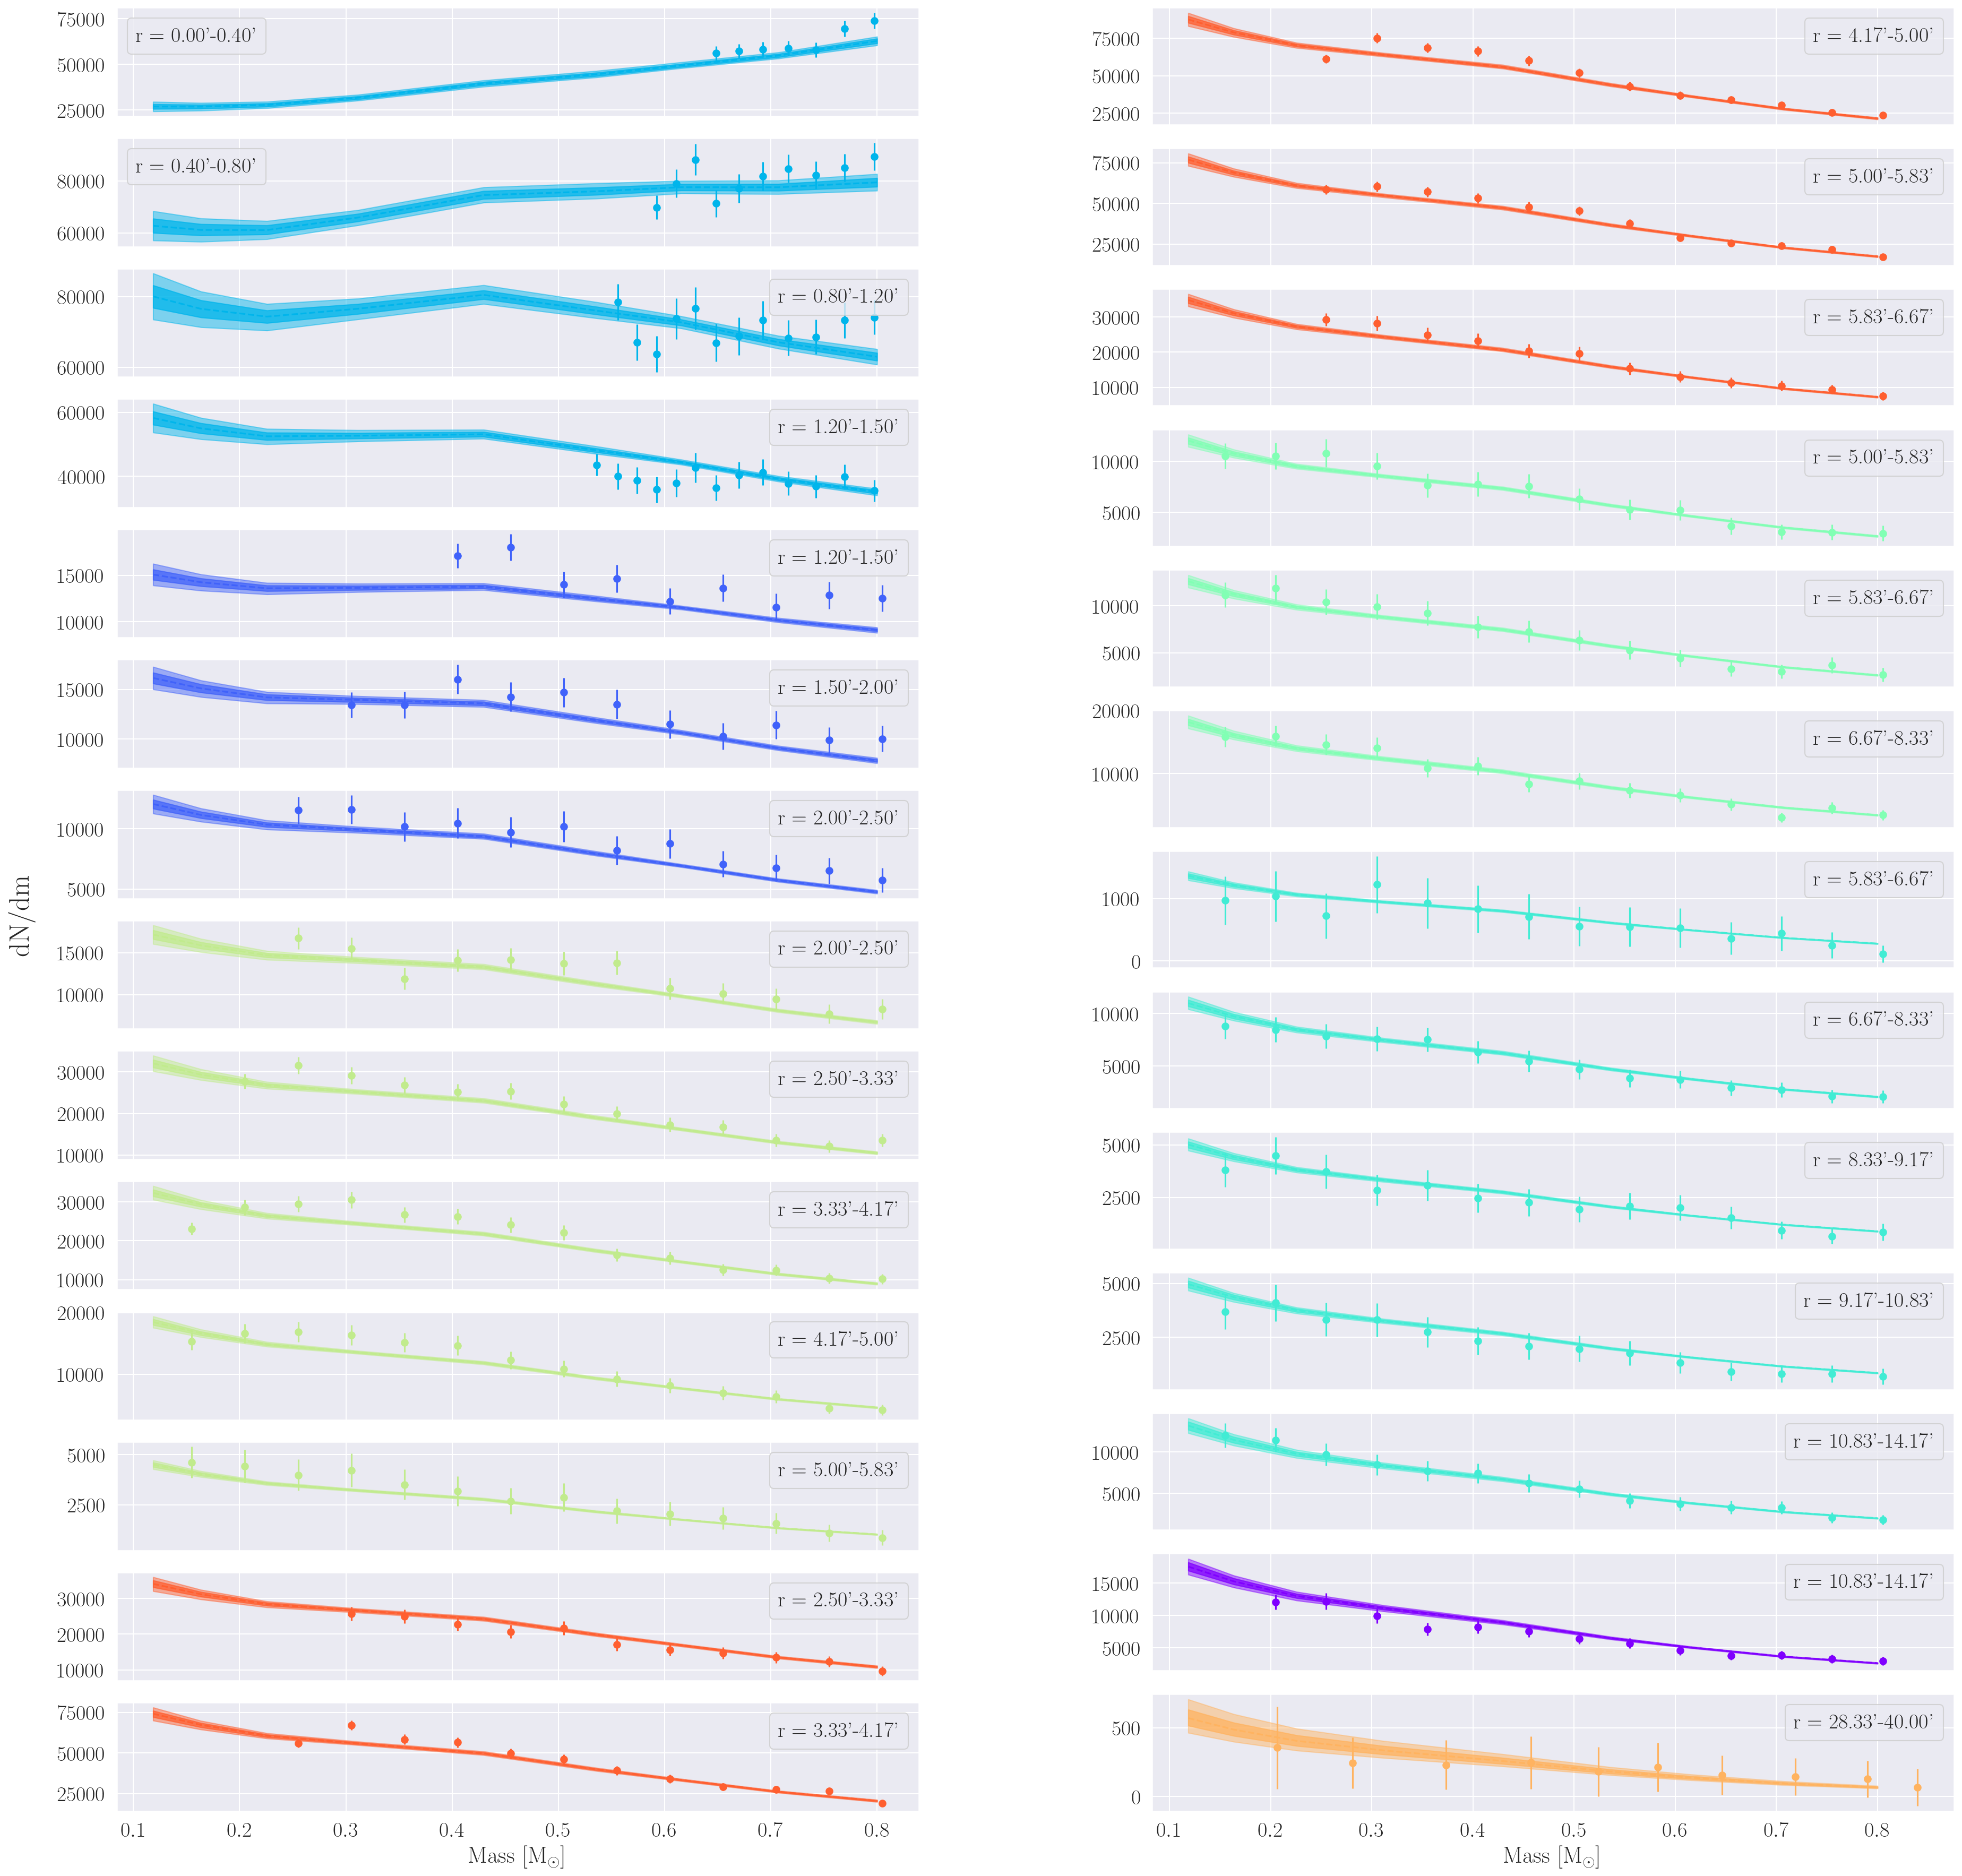
\includegraphics[width=0.8\textwidth]{figures/high_bin_model/mass_fun.png}
	\caption{Model fits to the stellar mass function data for models with a $10\%$ binary fraction.}
	\label{fig:highbin_mass_fun}
\end{figure}